\documentclass[UTF8]{article}
\usepackage{amsmath}
\usepackage{amssymb}
\usepackage{CTEX}
\usepackage{geometry}
\usepackage{graphicx}
\geometry{left=3.5cm,right=3.5cm,top=3.5cm,bottom=4cm}
%\title{Flame介绍文档}
%\author{Yiming Xia}
\begin{document}
\tableofcontents
\newpage
{\songti \noindent更新日志\\}%\noindent是取消缩进
{\songti
2018.07.02 介绍文档的latex文档建立

2018.07.15 更新对能量求导的推导,稍有遗忘,以及细节证明的缺漏,已补上

2018.07.18 以推广的眼光看MPM,需要补充图片说明
}

\newpage
\section{{序言}}

{\songti
人总是容易遗忘,在Flame构建的过程中我深有体会。有很多接口为了实现某一特殊功能而写,但是在后面看到这些接口的时候却发现自己忘了当时为什么要写这个接口,只能回头看代码。过程中,也有一些理论,前面在纸上推导过了,但是没有去实现,导致后面用到时,基本遗忘了当时的推导过程,从凌乱的草稿纸中寻找以前的推导思路,非常麻烦。从上面的两件事中,我意识到,做事情不光需要有阶段性的计划,也要有阶段性的总结,积淀。这种积淀,积累一方面是便于自己后续的发力,另一方面,也使得知识的传承变得更加容易。这篇文档就是以此为目标而写的。

Flame是我本科做毕业设计时,在完成毕业设计的任务后总结出的一个流体模拟框架。做流体框架的想法在做毕设的一开始就想好的,主要是因为在一些调研后,我发现,很多人写的流体模拟框架似乎并不好用,存在装配困难,平台局限,算法并不全等等问题,同时,由于毕设所用的物质点法天然就有着框架潜力,而且,在做毕设的过程中,我依次实现了弹性体,雪,水,沙子的模拟。所以,我尝试了将这些已有的代码进行封装,进行了集成,也就形成了Flame的雏形。

Flame的中文释义是:火焰,情人,激情。我取这个名字,一方面是因为我觉得像暴雪,寒霜这些名字都给人一种冰冷的感觉,起一个能给人温暖感觉的名字稍稍有点新意,另一方面,是觉得自己在大学四年实在是没能做出什么能让自己为之一振的事,希望能以此燃起自己心中的斗志。同时,因为硕士阶段自己可能不一定还能继续在这个方向上做,但是,为这个框架我自己付出了太多的努力,如果因为硕士阶段方向的问题而中途放弃不做的话,实在是让人觉得可惜,所以,希望能将这种劲头、激情保持住,坚定地走下去。

这个介绍文档记录了物质点法的算法推导,框架API。采用从乱序到有序,先随性后整理的方式写出。

学贵以恒,即便一路中遇到了低谷,懈怠,也要咬着牙挺过去。坚持下去,就能做出更好的结果。
}


\newpage
\section{{物质点法算法原理}}
\subsection{{运动描述}}
{\songti 模拟物质的运动,需要从物质的描述开始。所谓运动描述,即是一种映射关系,如图1,被研究的物质在初始时刻$t_0$所占的区域为$\Omega^0$,在其中选取一点$\textbf{\emph{X}}$,经过一段时间$t$的演化,物质所占区域由$\Omega^0$变为$\Omega^t$,点$\textbf{\emph{X}}$演化到点$\textbf{\emph{x}}$,从而,由$t_0$到$t$。在流体力学中,对于物质运动有两种描述方式,分别是:拉格朗日视角以及欧拉视角。“横看成岭侧成峰”,两种视角可以理解为对同一事物的不同看法。}


\begin{figure}[ht]

\centering
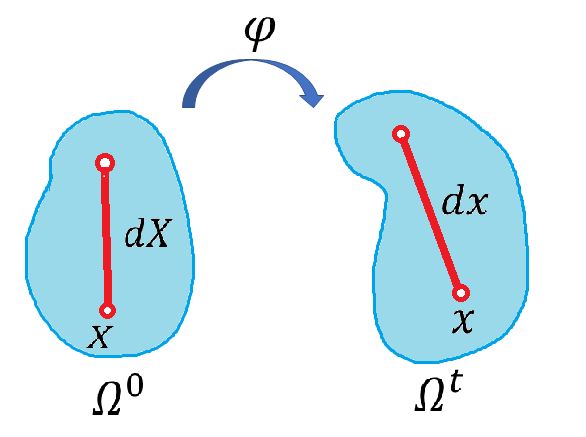
\includegraphics[scale=0.6]{chapter1/1.png}
\caption{映射关系}
\label{fig:label}
\end{figure}

\subsection{{从粒子到格点}}
{\songti 记粒子位置为$x_p$,格点的位置为$x_i$,格点到粒子间的插值函数记为$w_{ip}$,对插值函数有如下要求,$\sum_{i}w_{ip}=1$,因此,插值函数有多种选择,同时格点位置分布也可以有多种选择,常见的是规则分布的网格,如图所示,另外格点分布也可以是交错格点,如图,即MAC形式。
}
\subsubsection{{速度}}
{\songti 为满足插值前后动量守恒,这里使用粒子动量插值计算格点动量,
}

\section{{本构模型公式推导}}
\subsection{{弹性形变中用到的能量密度}}
{\songti Neo-Hookean弹性能量密度的表达形式是:\begin{equation}\Psi(F)=\mu \|F-R\|^2_F+\frac{\lambda}{2}(J-1)^2\end{equation}

其中,$J=det(F)$,$R$是对$F$进行极分解$F=RS$得到的结果。下面对其进行求导,计算$\frac{\partial \Psi(F)}{\partial F}$。

首先是矩阵的行列式对矩阵求导,由行列式的性质,可以得到,$F^{-1}=\frac{F^*}{det(F)}=J$,$F^*$是伴随矩阵。因此,$FF^*=det(F)I$,推得$\sum_{k}F_{ik}F^*_{ki}=det(F)$,$i$是0~N中的任意一个,我们用该展开形式进行求导计算,求出子项$\frac{\partial J}{\partial F_{ik}}$。由伴随矩阵的性质,$F_{ik}$与$F^*_{kj}$无关。这使得求导时,不用考虑耦合的问题。所以$\frac{\partial J}{\partial F_{ik}}=F^*_{ki}$,即$\frac{\partial J}{\partial F}={F^*}^{-T}=JF^{-T}$。

其次是对二阶范数$\|F-R\|^2_F$的求导,记$f=\|F-R\|^2_F$,根据二阶范数的定义$f=tr((F-R)^T(F-R))$,所以,\begin{equation}\delta f=\delta tr((F-R)^T(F-R))=\delta tr(F^TF-R^TF-F^TR+I)=2tr(F^T\delta F)-2tr(\delta S)\end{equation}下面列出一些推导中需要的引理:

(1)$tr(A^TB)=A:B$其中“$:$”是双点积,

(2)$\frac{\partial tr(A^TB)}{\partial B}=A$

(3)因为$\delta F=\delta RS+R\delta S$,所以$R^T\delta F=R^T\delta RS+\delta S$,$\delta S=R^T\delta RS+R^T\delta F$,$tr(\delta S)=tr(R^T\delta RS)+tr(R^T\delta F)$。因为$R^TR=I$,所以,$\delta R^TR+R^T\delta R=0$,因此,$R^T\delta R$是反对称阵。又$S$是对称阵,所以$tr(R^T\delta RS)=0$。此性质证明如下:设$A^T=A$,$B^T=-B$,$tr(AB)=tr(BA)=tr(A^TB^T)=-tr(AB)$,所以$tr(AB)=0$。所以$tr(\delta S)=0+tr(R^T\delta F)=tr(R^T\delta F)$

由(3)可得,$\delta f=2tr(F^T\delta F)-2tr(R^T\delta F)$。结合(1)(2)得,$\frac{\partial f}{\partial F}=2(F-R)$。

综上所述,\begin{equation}\frac{\partial \Psi(F)}{\partial F}=\mu \frac{\partial f}{\partial F}+\lambda(J-1)\frac{\partial J}{\partial F}=2\mu (F-R)+\lambda(J-1)JF^{-T}\end{equation}
}

\subsection{{弹塑性形变中用到的能量密度}}
{\songti Venant-Kirchhoff 弹性能量密度的表达形式是:\begin{equation}\Psi(F)=\mu tr((ln\Sigma)^2)+\frac{1}{2}\lambda(tr(ln\Sigma))^2\end{equation}
式中$ln\Sigma$仅对对角项作用。下面求$\frac{\partial \Psi(F)}{\partial F}$
}
%\begin{equation}
%分隔一个过长的公式分行显示使用split环境
%\begin{split}
%arg \min_{\substack{\Theta, W}} L_{feedback}+L_{content}  =
%& - \sum_{\left(m,i,j\right) \in D_s} \ln f \left( r_{mij}\right) + \lambda\|\theta\|^2\\
%& + \|A^eW^e-Y^e\|^2_F + \frac 12 \sum_{e\in \{u,v\}}\lambda^e\|W^e\|^2_F
%\end{split}
%\end{equation}

\end{document} 